\section{Implementation and artifact contracts}
The source files \texttt{src/piml/s2.py} and \texttt{tests/test\_s2.py} implement the successor and its numerical checks. Legacy S1 source, tests, configs and raw development evidence are preserved under \texttt{evidence/s1}; \texttt{SHA256.json} binds those files byte for byte. The active legacy report formatter receives only a Python 3.11 syntax compatibility repair; the archived source is unchanged.

Each S2 run retains \texttt{config.json}, \texttt{source\_manifest.json}, \texttt{environment.json}, \texttt{cases.jsonl}, \texttt{metrics.jsonl}, \texttt{models.json}, \texttt{offline\_costs.json}, \texttt{analysis.json}, \texttt{receipt.json}, \texttt{progress.json}, a file manifest and verification receipt. An unsuccessful execution additionally retains a failure record and available partial measurements. Output directories are never overwritten.

\section{Reproduction commands}
From the project directory, install the research extra and use one thread:
\begin{verbatim}
python -m pip install '.[research]'
export OPENBLAS_NUM_THREADS=1 OMP_NUM_THREADS=1
export MKL_NUM_THREADS=1 PYTHONPATH=src
python -m unittest discover -s tests -v
python -m piml verify evidence/s1/development-S1-v1
python -m piml.s2 run configs/s2_development.json NEW_DEV_DIR
python -m piml.s2 verify NEW_DEV_DIR
\end{verbatim}
Confirmatory execution additionally requires the frozen configuration and source receipt. Use a new output directory for an explicitly labeled replication; never present a second run as a new independent protected experiment. Exact delivery and artifact hashes are recorded in the release ledger rather than inferred from the presence of these commands.

\section{Adversarial checks and claim mapping}
The flaw register covers endpoint saturation, direct-solver competitiveness, weak classical controls, prior art, structural misspecification, repeated factorization, recursive-residual drift, invalid uncertainty claims, timing order, training replication, multiplicity, semantic verification, provenance, packaging, resources, synthetic scope, shared reference code, unequal capacity, source drift and independent reproduction. A fix is accepted only when its stated evidence exists. The machine-readable claim ledger maps every retained numerical statement to its run, analysis and rendered table. Proofs establish only SPD, spectral equivalence and source superposition, not learned performance.

\section{Complete S2 matrix}
\small
\begin{longtable}{rlllrrr}
\toprule
$N$ & $\tau$ & Regime & Method & Iterations & ms & Failures \\
\midrule\endhead
65 & 1e-06 & IID & Direct Thomas & 0.00 & 0.245 & 0 \\
65 & 1e-06 & IID & Zero + Jacobi & 62.89 & 1.630 & 0 \\
65 & 1e-06 & IID & Quadratic + Jacobi & 62.97 & 1.716 & 0 \\
65 & 1e-06 & IID & Zero + Laplacian & 12.22 & 1.778 & 0 \\
65 & 1e-06 & IID & Physics + Laplacian & 11.24 & 1.888 & 0 \\
65 & 1e-06 & IID & Quadratic + Laplacian & 10.21 & 1.596 & 0 \\
65 & 1e-06 & IID & Degree 1 + Laplacian & 10.07 & 1.560 & 0 \\
65 & 1e-06 & IID & Structured + Laplacian & 8.96 & 1.435 & 0 \\
65 & 1e-06 & IID & Shuffled + Laplacian & 12.39 & 1.873 & 0 \\
65 & 1e-06 & coeff. OOD & Direct Thomas & 0.00 & 0.248 & 0 \\
65 & 1e-06 & coeff. OOD & Zero + Jacobi & 62.91 & 1.639 & 0 \\
65 & 1e-06 & coeff. OOD & Quadratic + Jacobi & 63.00 & 1.727 & 0 \\
65 & 1e-06 & coeff. OOD & Zero + Laplacian & 21.44 & 2.955 & 0 \\
65 & 1e-06 & coeff. OOD & Physics + Laplacian & 20.51 & 3.078 & 0 \\
65 & 1e-06 & coeff. OOD & Quadratic + Laplacian & 19.59 & 2.813 & 0 \\
65 & 1e-06 & coeff. OOD & Degree 1 + Laplacian & 19.42 & 2.751 & 0 \\
65 & 1e-06 & coeff. OOD & Structured + Laplacian & 18.19 & 2.642 & 0 \\
65 & 1e-06 & coeff. OOD & Shuffled + Laplacian & 22.36 & 3.150 & 0 \\
65 & 1e-06 & source OOD & Direct Thomas & 0.00 & 0.245 & 0 \\
65 & 1e-06 & source OOD & Zero + Jacobi & 62.92 & 1.633 & 0 \\
65 & 1e-06 & source OOD & Quadratic + Jacobi & 62.99 & 1.714 & 0 \\
65 & 1e-06 & source OOD & Zero + Laplacian & 12.19 & 1.769 & 0 \\
65 & 1e-06 & source OOD & Physics + Laplacian & 11.21 & 1.882 & 0 \\
65 & 1e-06 & source OOD & Quadratic + Laplacian & 11.34 & 1.748 & 0 \\
65 & 1e-06 & source OOD & Degree 1 + Laplacian & 11.36 & 1.723 & 0 \\
65 & 1e-06 & source OOD & Structured + Laplacian & 11.32 & 1.732 & 0 \\
65 & 1e-06 & source OOD & Shuffled + Laplacian & 12.30 & 1.868 & 0 \\
65 & 1e-10 & IID & Direct Thomas & 0.00 & 0.247 & 0 \\
65 & 1e-10 & IID & Zero + Jacobi & 63.00 & 1.634 & 0 \\
65 & 1e-10 & IID & Quadratic + Jacobi & 63.00 & 1.719 & 0 \\
65 & 1e-10 & IID & Zero + Laplacian & 18.74 & 2.610 & 0 \\
65 & 1e-10 & IID & Physics + Laplacian & 17.74 & 2.712 & 0 \\
65 & 1e-10 & IID & Quadratic + Laplacian & 16.91 & 2.444 & 0 \\
65 & 1e-10 & IID & Degree 1 + Laplacian & 16.80 & 2.408 & 0 \\
65 & 1e-10 & IID & Structured + Laplacian & 15.68 & 2.281 & 0 \\
65 & 1e-10 & IID & Shuffled + Laplacian & 18.93 & 2.706 & 0 \\
65 & 1e-10 & coeff. OOD & Direct Thomas & 0.00 & 0.249 & 0 \\
65 & 1e-10 & coeff. OOD & Zero + Jacobi & 63.00 & 1.646 & 0 \\
65 & 1e-10 & coeff. OOD & Quadratic + Jacobi & 63.00 & 1.736 & 0 \\
65 & 1e-10 & coeff. OOD & Zero + Laplacian & 31.10 & 4.201 & 0 \\
65 & 1e-10 & coeff. OOD & Physics + Laplacian & 30.19 & 4.319 & 0 \\
65 & 1e-10 & coeff. OOD & Quadratic + Laplacian & 29.35 & 4.067 & 0 \\
65 & 1e-10 & coeff. OOD & Degree 1 + Laplacian & 29.21 & 4.017 & 0 \\
65 & 1e-10 & coeff. OOD & Structured + Laplacian & 28.12 & 3.893 & 0 \\
65 & 1e-10 & coeff. OOD & Shuffled + Laplacian & 31.91 & 4.398 & 0 \\
65 & 1e-10 & source OOD & Direct Thomas & 0.00 & 0.250 & 0 \\
65 & 1e-10 & source OOD & Zero + Jacobi & 63.00 & 1.645 & 0 \\
65 & 1e-10 & source OOD & Quadratic + Jacobi & 63.00 & 1.724 & 0 \\
65 & 1e-10 & source OOD & Zero + Laplacian & 18.84 & 2.622 & 0 \\
65 & 1e-10 & source OOD & Physics + Laplacian & 17.86 & 2.723 & 0 \\
65 & 1e-10 & source OOD & Quadratic + Laplacian & 18.02 & 2.596 & 0 \\
65 & 1e-10 & source OOD & Degree 1 + Laplacian & 18.02 & 2.562 & 0 \\
65 & 1e-10 & source OOD & Structured + Laplacian & 17.99 & 2.581 & 0 \\
65 & 1e-10 & source OOD & Shuffled + Laplacian & 18.96 & 2.717 & 0 \\
129 & 1e-06 & IID & Direct Thomas & 0.00 & 0.448 & 0 \\
129 & 1e-06 & IID & Zero + Jacobi & 126.07 & 3.246 & 0 \\
129 & 1e-06 & IID & Quadratic + Jacobi & 126.96 & 3.360 & 0 \\
129 & 1e-06 & IID & Zero + Laplacian & 12.56 & 3.212 & 0 \\
129 & 1e-06 & IID & Physics + Laplacian & 11.56 & 3.393 & 0 \\
129 & 1e-06 & IID & Quadratic + Laplacian & 10.54 & 2.853 & 0 \\
129 & 1e-06 & IID & Degree 1 + Laplacian & 10.43 & 2.789 & 0 \\
129 & 1e-06 & IID & Structured + Laplacian & 9.13 & 2.518 & 0 \\
129 & 1e-06 & IID & Shuffled + Laplacian & 12.62 & 3.326 & 0 \\
129 & 1e-06 & coeff. OOD & Direct Thomas & 0.00 & 0.453 & 0 \\
129 & 1e-06 & coeff. OOD & Zero + Jacobi & 126.34 & 3.265 & 0 \\
129 & 1e-06 & coeff. OOD & Quadratic + Jacobi & 126.96 & 3.372 & 0 \\
129 & 1e-06 & coeff. OOD & Zero + Laplacian & 24.33 & 5.950 & 0 \\
129 & 1e-06 & coeff. OOD & Physics + Laplacian & 23.33 & 6.103 & 0 \\
129 & 1e-06 & coeff. OOD & Quadratic + Laplacian & 22.14 & 5.521 & 0 \\
129 & 1e-06 & coeff. OOD & Degree 1 + Laplacian & 21.88 & 5.436 & 0 \\
129 & 1e-06 & coeff. OOD & Structured + Laplacian & 20.41 & 5.129 & 0 \\
129 & 1e-06 & coeff. OOD & Shuffled + Laplacian & 25.56 & 6.303 & 0 \\
129 & 1e-06 & source OOD & Direct Thomas & 0.00 & 0.454 & 0 \\
129 & 1e-06 & source OOD & Zero + Jacobi & 126.19 & 3.264 & 0 \\
129 & 1e-06 & source OOD & Quadratic + Jacobi & 126.92 & 3.366 & 0 \\
129 & 1e-06 & source OOD & Zero + Laplacian & 11.90 & 3.089 & 0 \\
129 & 1e-06 & source OOD & Physics + Laplacian & 10.91 & 3.248 & 0 \\
129 & 1e-06 & source OOD & Quadratic + Laplacian & 11.09 & 2.981 & 0 \\
129 & 1e-06 & source OOD & Degree 1 + Laplacian & 11.09 & 2.951 & 0 \\
129 & 1e-06 & source OOD & Structured + Laplacian & 11.04 & 2.961 & 0 \\
129 & 1e-06 & source OOD & Shuffled + Laplacian & 12.03 & 3.206 & 0 \\
129 & 1e-10 & IID & Direct Thomas & 0.00 & 0.454 & 0 \\
129 & 1e-10 & IID & Zero + Jacobi & 127.00 & 3.309 & 0 \\
129 & 1e-10 & IID & Quadratic + Jacobi & 127.00 & 3.411 & 0 \\
129 & 1e-10 & IID & Zero + Laplacian & 19.48 & 4.826 & 0 \\
129 & 1e-10 & IID & Physics + Laplacian & 18.49 & 5.036 & 0 \\
129 & 1e-10 & IID & Quadratic + Laplacian & 17.46 & 4.450 & 0 \\
129 & 1e-10 & IID & Degree 1 + Laplacian & 17.33 & 4.406 & 0 \\
129 & 1e-10 & IID & Structured + Laplacian & 16.12 & 4.147 & 0 \\
129 & 1e-10 & IID & Shuffled + Laplacian & 19.56 & 4.934 & 0 \\
129 & 1e-10 & coeff. OOD & Direct Thomas & 0.00 & 0.464 & 0 \\
129 & 1e-10 & coeff. OOD & Zero + Jacobi & 127.00 & 3.303 & 0 \\
129 & 1e-10 & coeff. OOD & Quadratic + Jacobi & 127.00 & 3.398 & 0 \\
129 & 1e-10 & coeff. OOD & Zero + Laplacian & 36.76 & 8.796 & 0 \\
129 & 1e-10 & coeff. OOD & Physics + Laplacian & 35.76 & 8.980 & 0 \\
129 & 1e-10 & coeff. OOD & Quadratic + Laplacian & 34.73 & 8.426 & 0 \\
129 & 1e-10 & coeff. OOD & Degree 1 + Laplacian & 34.50 & 8.372 & 0 \\
129 & 1e-10 & coeff. OOD & Structured + Laplacian & 33.09 & 8.074 & 0 \\
129 & 1e-10 & coeff. OOD & Shuffled + Laplacian & 37.89 & 9.148 & 0 \\
129 & 1e-10 & source OOD & Direct Thomas & 0.00 & 0.454 & 0 \\
129 & 1e-10 & source OOD & Zero + Jacobi & 127.00 & 3.263 & 0 \\
129 & 1e-10 & source OOD & Quadratic + Jacobi & 127.00 & 3.368 & 0 \\
129 & 1e-10 & source OOD & Zero + Laplacian & 18.59 & 4.606 & 0 \\
129 & 1e-10 & source OOD & Physics + Laplacian & 17.62 & 4.795 & 0 \\
129 & 1e-10 & source OOD & Quadratic + Laplacian & 17.77 & 4.541 & 0 \\
129 & 1e-10 & source OOD & Degree 1 + Laplacian & 17.77 & 4.492 & 0 \\
129 & 1e-10 & source OOD & Structured + Laplacian & 17.70 & 4.497 & 0 \\
129 & 1e-10 & source OOD & Shuffled + Laplacian & 18.75 & 4.740 & 0 \\
\bottomrule\end{longtable}
\normalsize


\section{Final release verification and model flow}
\begin{figure}[ht]
\centering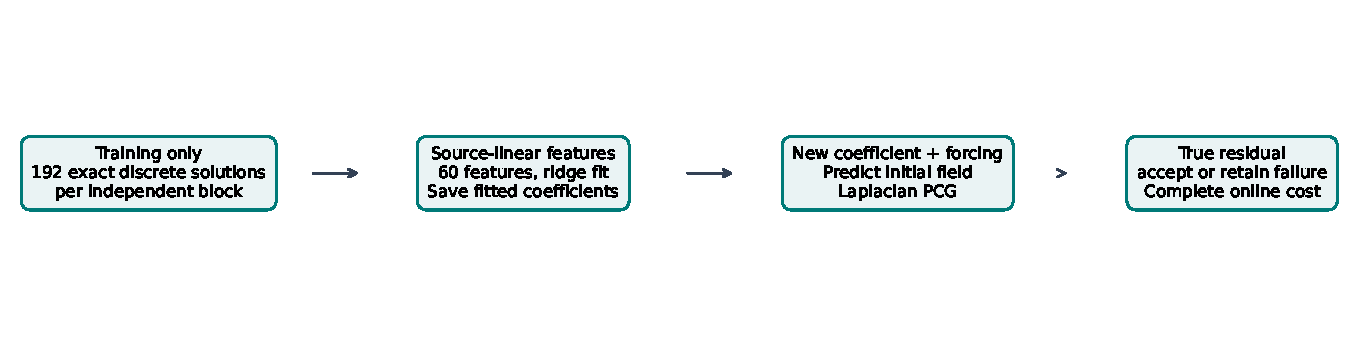
\includegraphics[width=\linewidth]{figures/pipeline.pdf}
\caption{Chronological model flow. Training and online evaluation use disjoint samples. The complete online path ends with explicit residual certification; no prediction is accepted on trust.}\label{fig:pipeline}
\end{figure}
A separate Kaggle release job installed the built wheel in a fresh virtual environment and passed all 26 tests. It replayed the full confirmation and ran an audit that imports no project solver code: SciPy's banded solver checked all 2,880 discrete targets, a separately assembled flux operator checked all 17,280 returned solutions, and all $5^5$ training-block bootstrap resamples independently reproduced the primary decision. The flux check allows an explicitly reported roundoff margin of $10^{-11}\max(\|b\|,1)$; it does not replace or relax the original strict acceptance gate. This is an independently implemented check by the same research agent, not reproduction by an independent investigator.

The final audit reports zero relative difference between the retained targets and SciPy's banded reference on these cases. Its exact finite-bootstrap interval against zero start is [27.28, 28.26]\%, compared with [27.28, 28.22]\% from the frozen Monte Carlo procedure. The physics-start interval is [20.94, 21.50]\% in both. The primary decision is unchanged; the frozen analysis is preserved.

\begin{table}[ht]
\centering\small
\begin{tabular}{lrrr}
\toprule
Model ($N=129$) & Parameters & Mean fit (ms) & Training generation (ms) \\
\midrule
Quadratic & 5715 & 14.275 & 191.543 \\
Source-linear degree 1 & 2540 & 8.361 & 191.543 \\
Source-linear degree 2 & 7620 & 13.562 & 191.543 \\
Shuffled source-linear & 7620 & 13.406 & 191.543 \\
\bottomrule
\end{tabular}
\caption{Offline cost across five training blocks. The same 192-example training set is shared by all models within a block; its generation cost is shown per model for comparability and must not be summed four times. Loading is excluded from both these fitting measurements and online timings. No amortized speed claim is made.}
\end{table}
